\chapter{Metodologia}

Neste capítulo, será descrito a visão geral a respeito do método de trabalho
que foi aplicado durante a elaboração do sistema e de como as tarefas a serem
desenvolvidas foram organizadas entre os integrantes do grupo.

Mesmo antes que a escolha em relação ao tema que seria desenvolvido durante o
ano fosse decidida, já havia um consenso de que a organização do trabalho a ser
aplicada se basearia na metodologia ágil.

A metodologia ágil é um conceito amplamente usado no mundo do desenvolvimento
de software, que utiliza o manifesto ágil ~\citet{agileManifesto} como base e
que, resumidamente, é constituído de um conjunto de práticas que visa uma
entrega contínua ao longo do projeto, que possibilite estruturar uma relação de
tarefas clara e intuitiva durante todo o processo, e que seja capaz de manter
todos os membros envolvidos alinhados quanto ao \textit{status} do
desenvolvimento.

A escolha pela metodologia ágil se deu pelo fato de que ambos os integrantes já
haviam tido contato com esse método de trabalho, sendo o primeiro deles a
partir da disciplina MAC0472 (Laboratório de Métodos Ágeis) e também utilizado
no desenvolvimento do projeto principal na disciplina MAC0413 (Tópicos
Avançados de Programação Orientada a Objetos).

Um dos tipos mais aplicados do conceito de metodologia ágil é o chamado
\textit{KanBan}. Como descrito por ~\citet{wakode2015overview}, esta prática se
baseia no uso de um quadro que é preenchido com diversos cartões que descrevem
como está o andamento do projeto. Neles ficam descritas atividades que deveriam
ser realizadas, destacando entre elas quais têm a maior prioridade; relatam
quais pontos estão sendo desenvolvidos no momento; além de também manterem
registros dos pontos que já foram entregues e, portanto, já estão implementados
no serviço.

Este trabalho usou o sistema do \textit{KanBan} como modelo para guiar o
processo de desenvolvimento. Para isto, foi utilizada a plataforma
\textit{Trello} onde, assim como descrito no último parágrafo, os
\textit{status} das tarefas foram mantidos e registrados ao longo do
desenvolvimento. O quadro com as tarefas pode ser acessado através do endereço
\href{https://trello.com/b/kGpOiOTE/tcc-eventos-usp}{https://trello.com/tcc-eventos-usp}.

\begin{figure}[h]
    \centering
    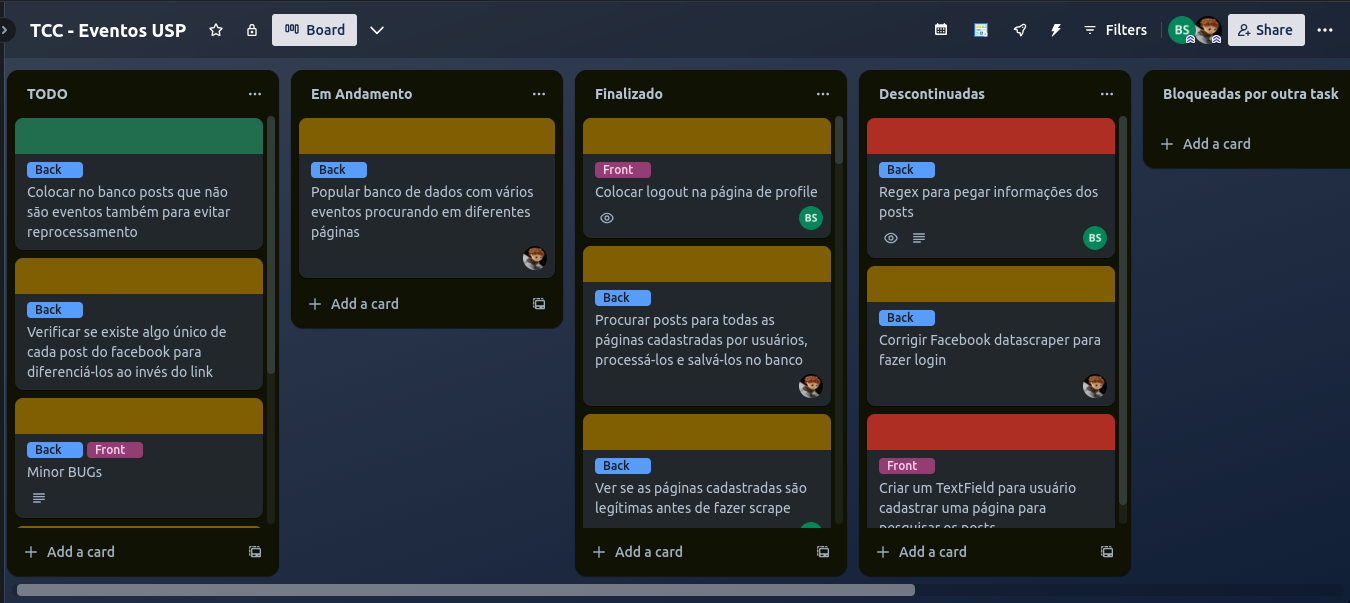
\includegraphics[width=1\textwidth]{figuras/trello.png}
    \caption{Quadro KanBan com as tarefas na plataforma Trello}
    \label{fig:enter-label}
\end{figure}

As tarefas a serem desenvolvidas foram separadas de acordo com seu escopo
dentro da divisão macro do sistema, isto é, eram classificadas como sendo
direcionadas ao \textit{back-end} e ao \textit{front-end}. Além disso, foi
feita uma classificação com relação à dificuldade de execução das tarefas a
partir de uma estimativa prévia, sendo essas consideradas fáceis (verde), médio
(amarelo) e difícil (vermelho).
